\begin{frame}{$\mathbb{P}^2(\mathbb{K})$}
    \begin{columns}
        \begin{column}{0.6\textwidth}
            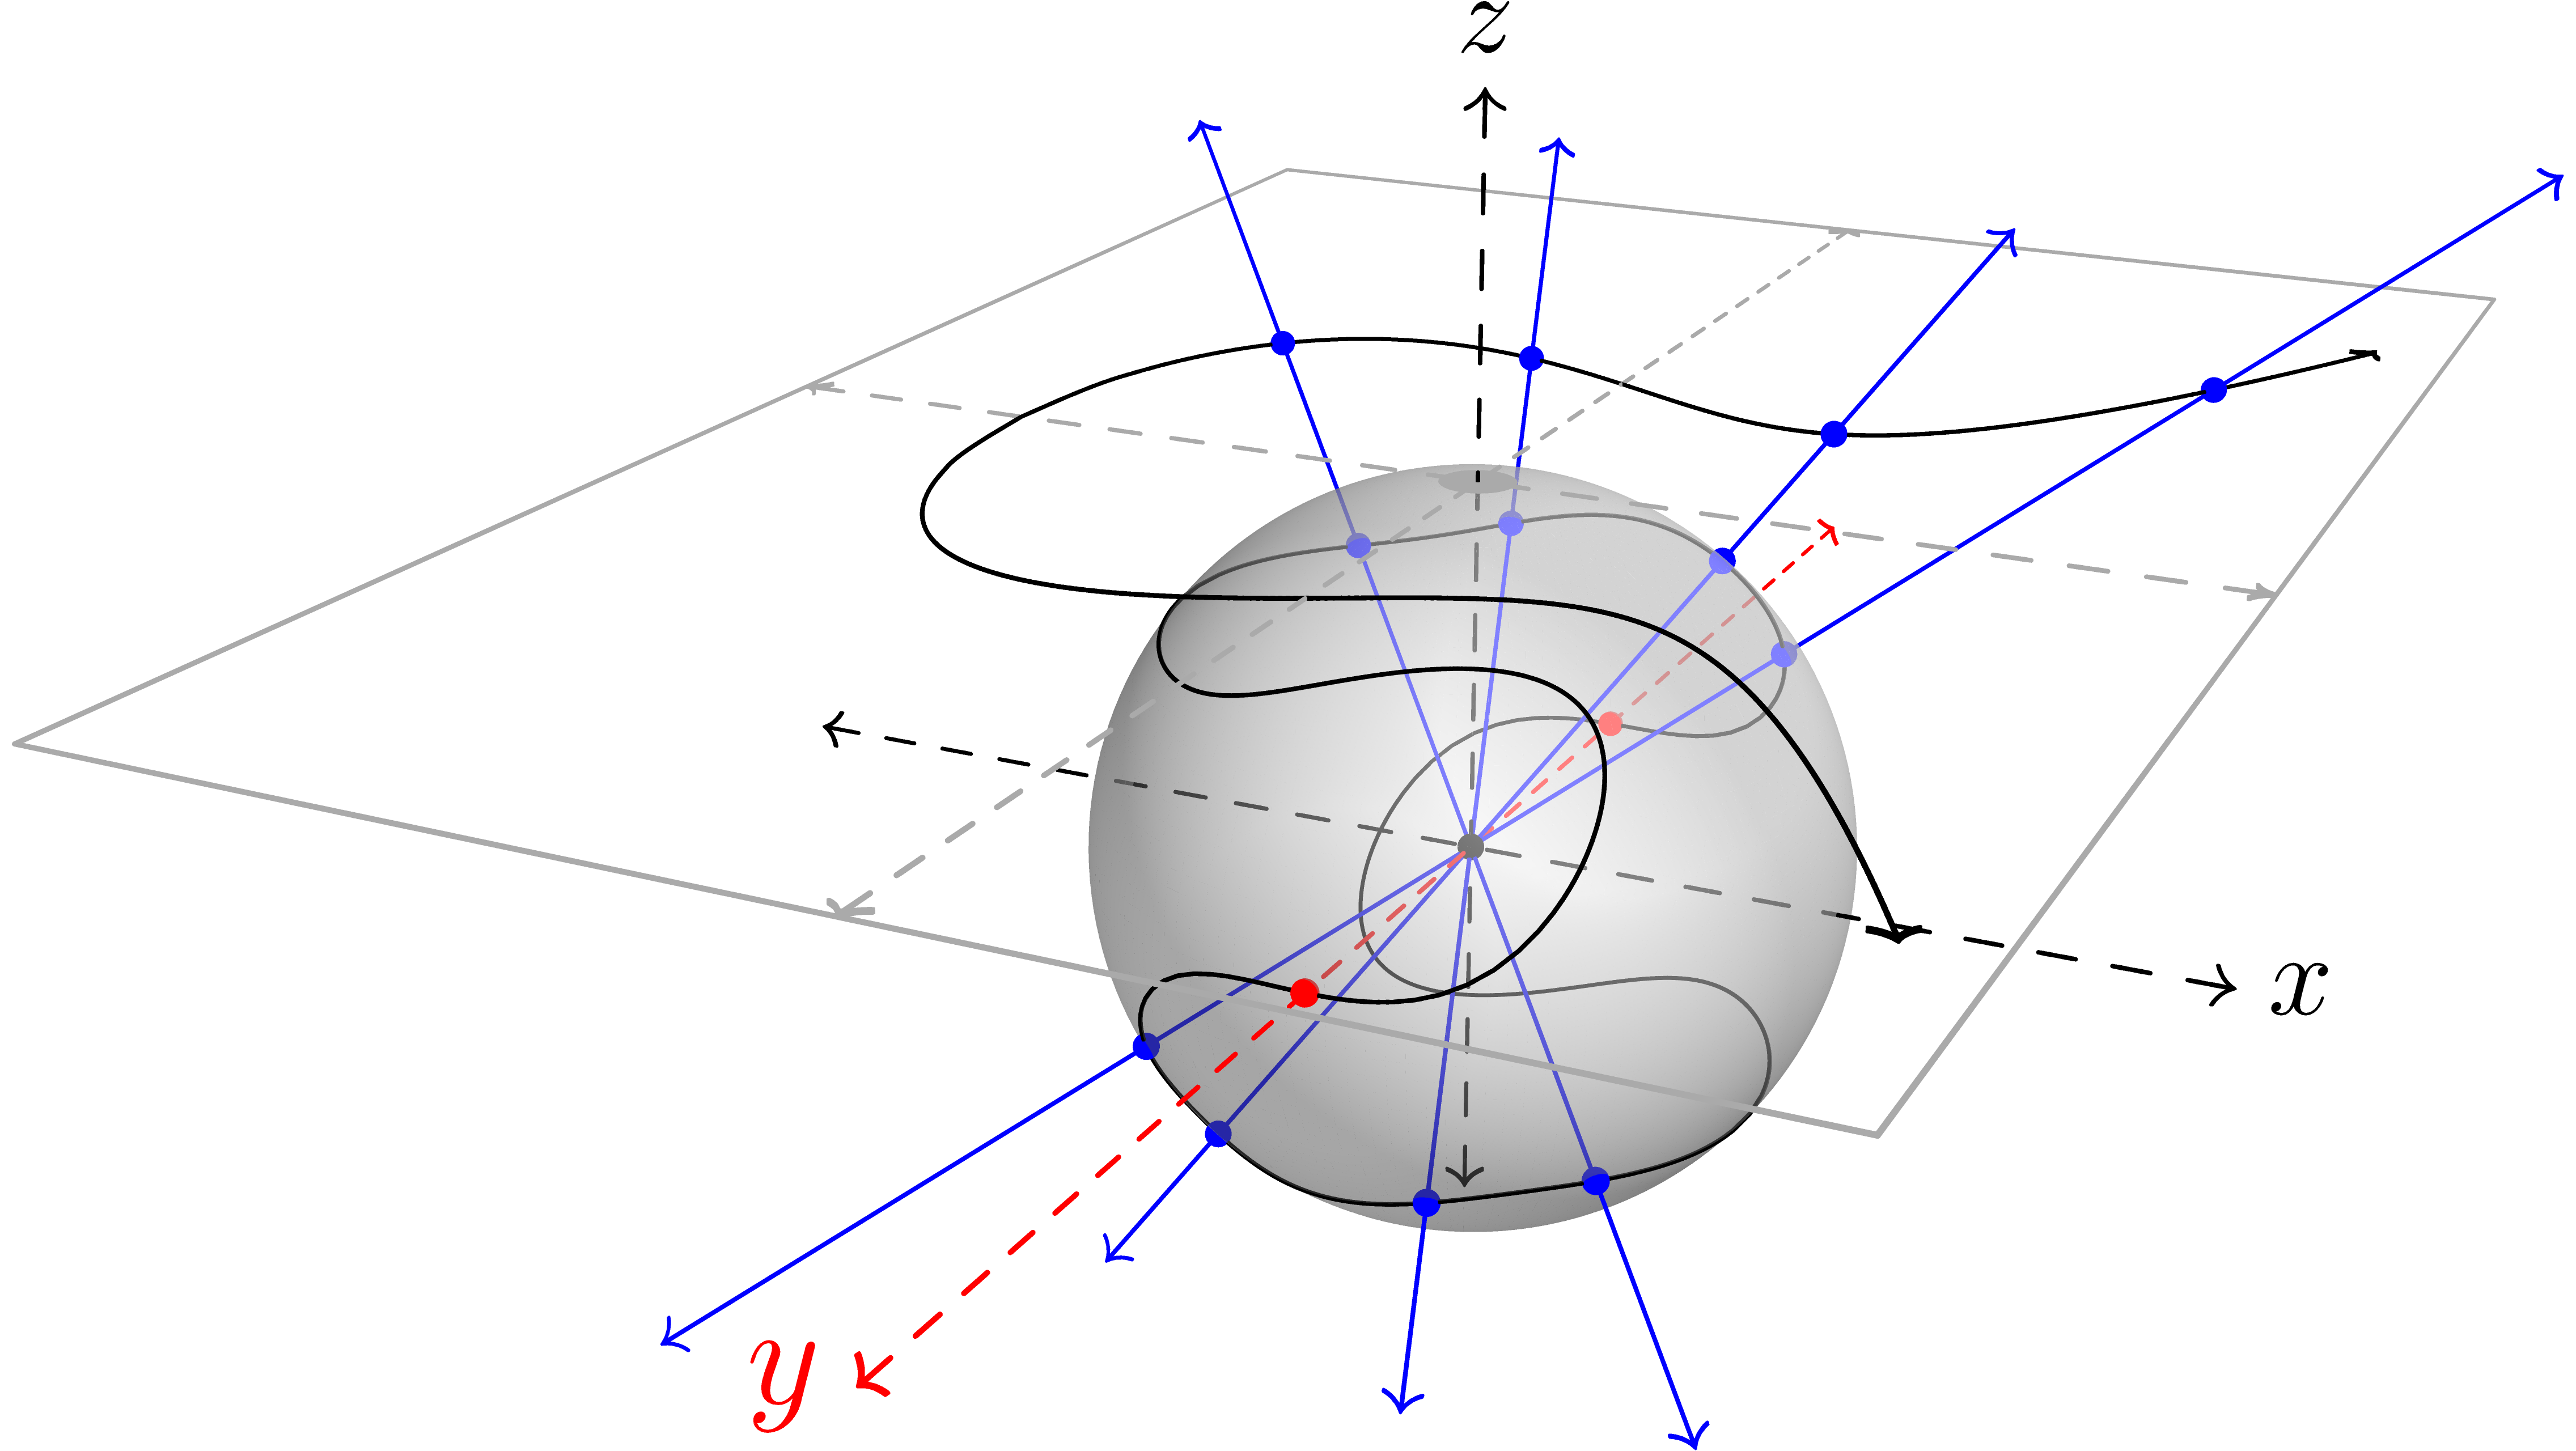
\includegraphics[width=\linewidth]{img/p^2.png}
        \end{column}
        \begin{column}{0.5\textwidth}
            \begin{definitionblock}{\\Projektiver Raum}
                \[
                    \mathbb{P}^n(\mathbb{K)} = \left( \mathbb{K}^{n+1} \setminus \{0\} \right) / \sim
                \]
                \begin{center}
                    mit der Äquivalenzrelation \\
                \end{center}
                \[
                    \sim: x \sim y \Leftrightarrow \exists \lambda \in \mathbb{K} \setminus \{0\} : x = \lambda y.
                \]
            \end{definitionblock}
            \vspace{1em}
            $P = (X:Y:Z) \in \mathbb{P}^2(\mathbb{K})$\\
            $(X:Y:Z)\sim(\lambda X:\lambda Y:\lambda Z)$
        \end{column}    
    \end{columns}
\end{frame}

\begin{frame}{$\mathbb{P}^2(\mathbb{K})$}
    \begin{columns}
        \begin{column}{0.6\textwidth}
            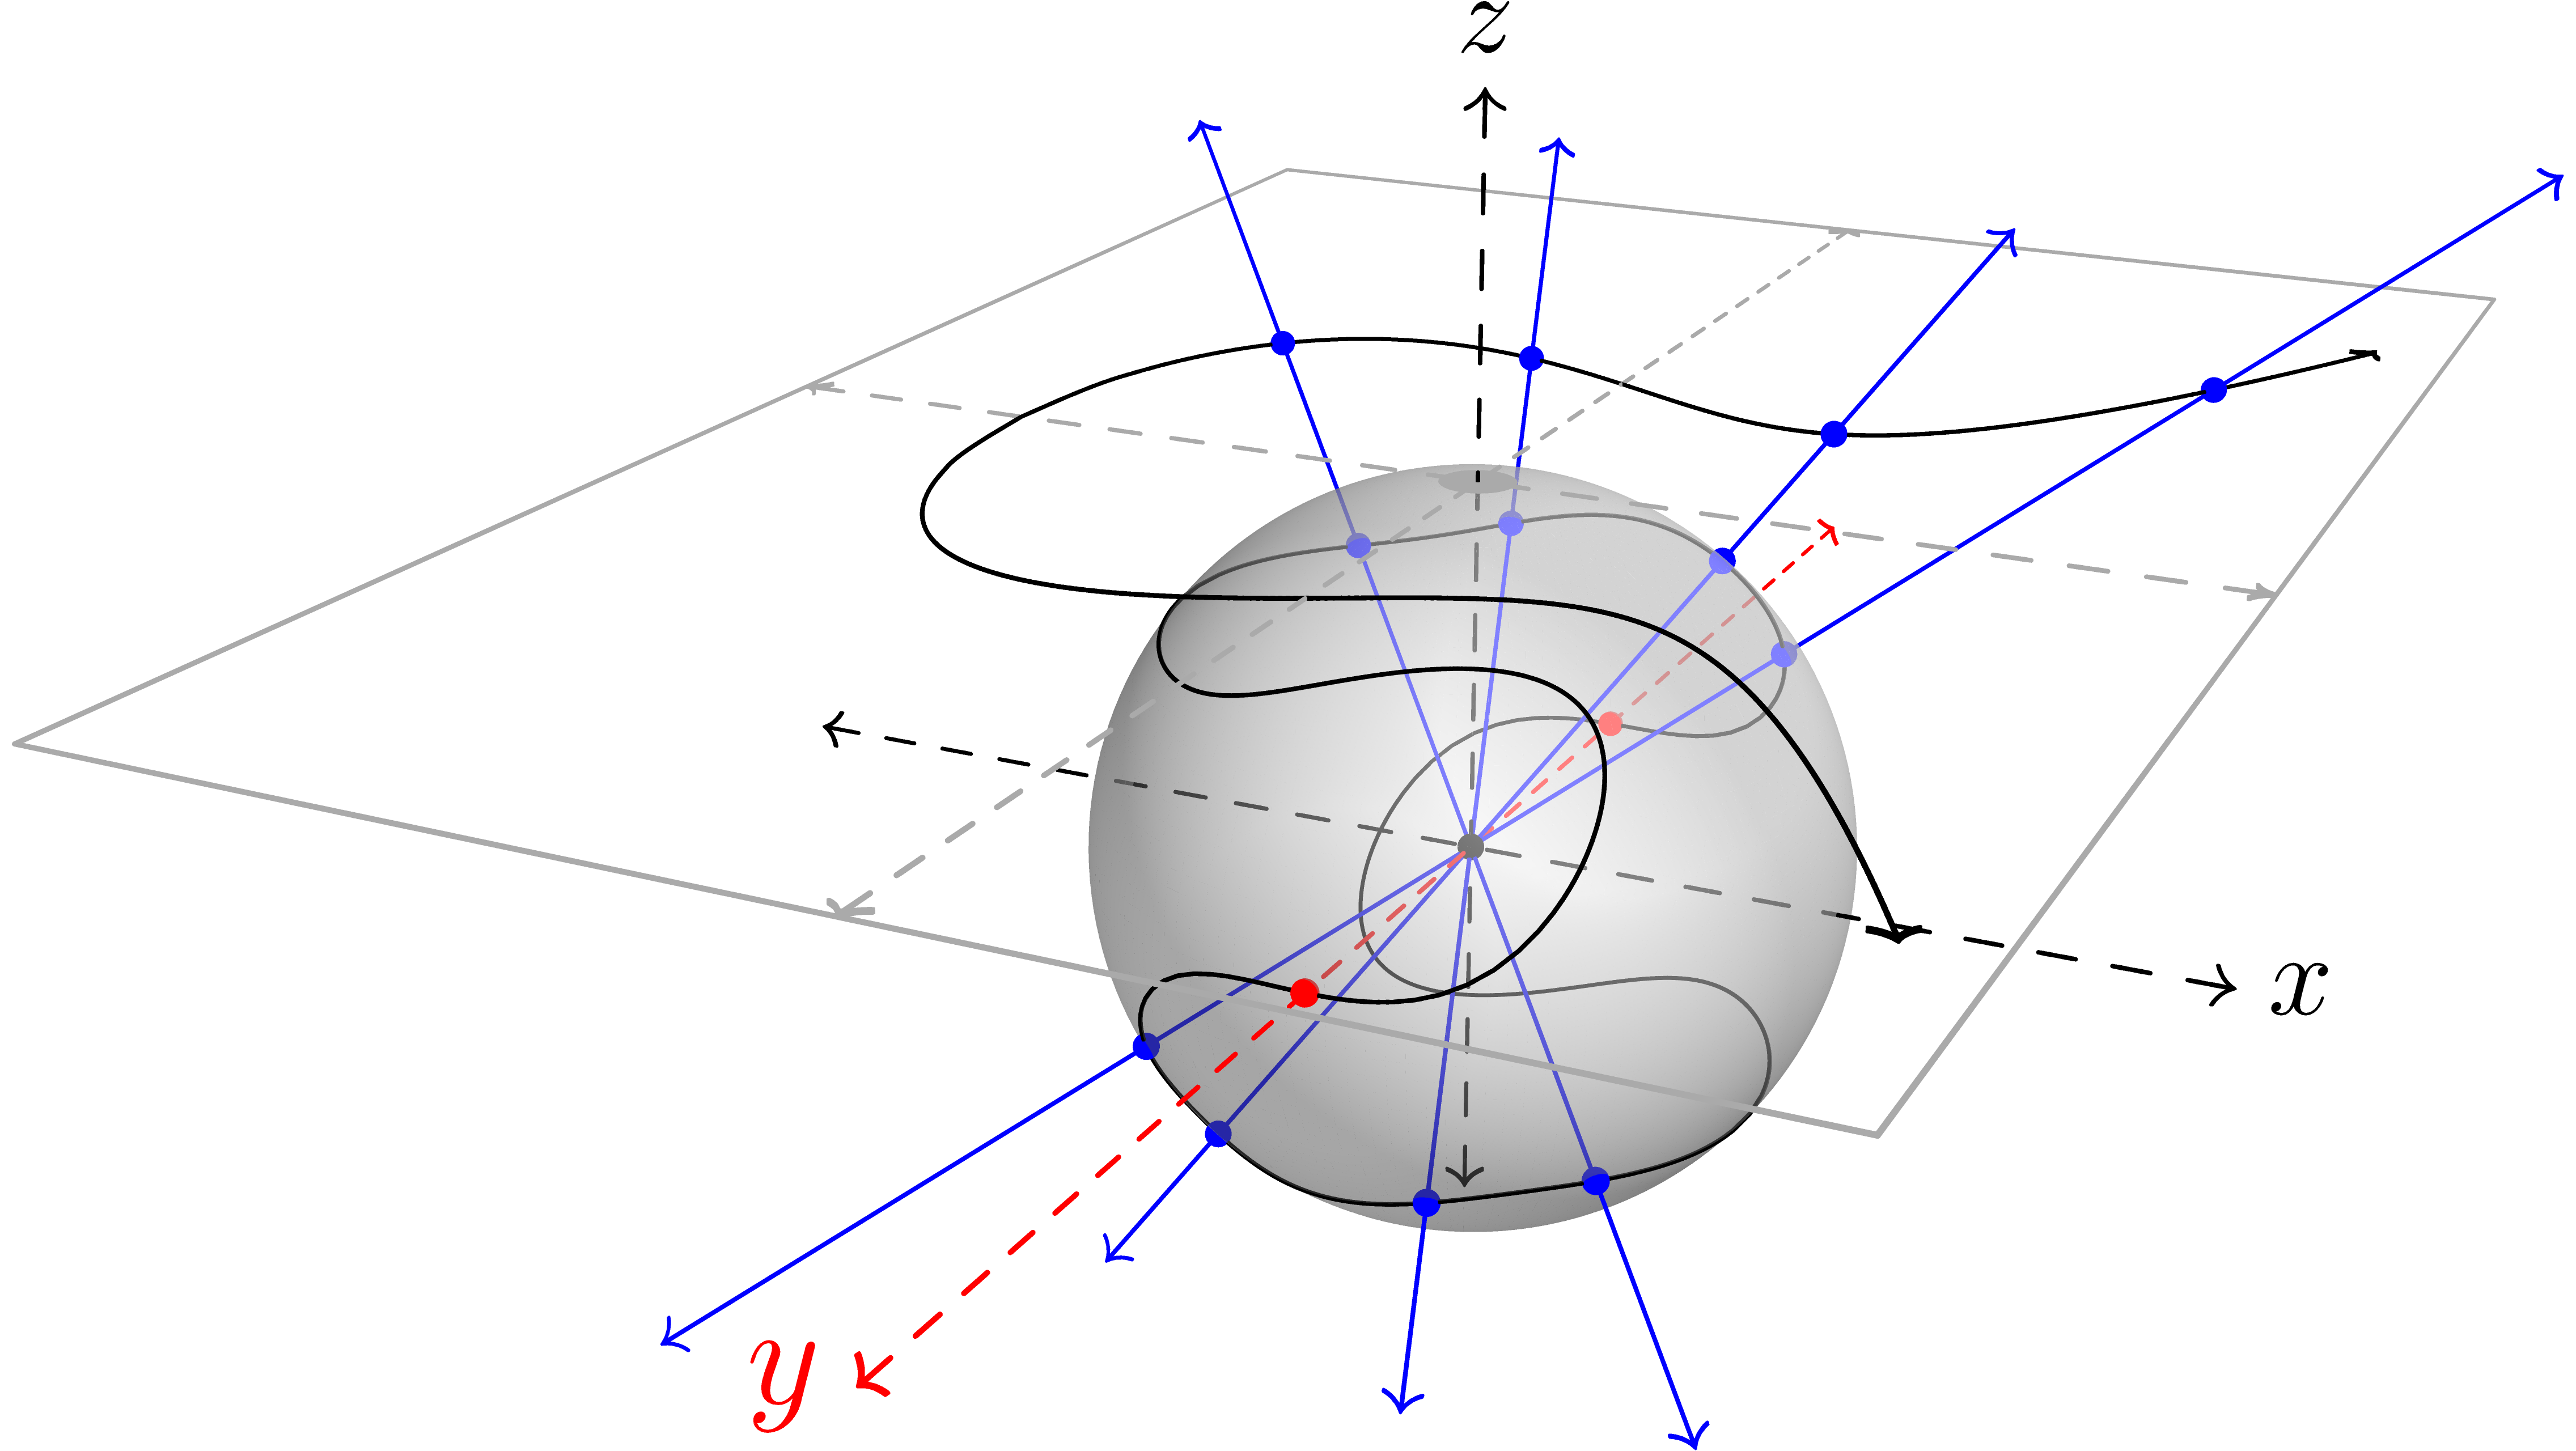
\includegraphics[width=\linewidth]{img/p^2.png}
        \end{column}
        \begin{column}{0.5\textwidth}
            \((x, y) = \left( \frac{X}{Z}, \frac{Y}{Z} \right)\)
            \[\mathcal{E}_{(A,B)}:BY^2Z=X^3+AX^2Z+XZ^2\subseteq\mathbb{P}^2\]
            \begin{algorithmblock}
                $(i)$ $Z\neq0$ \\ 
                \quad Alle Punkte der affinen Kurve liegen auf der Ebene $(x : y : 1)$\\
                $(ii)$ $Z=0\\0=X^3\Leftrightarrow X=0$ und Y beliebig\\$\mathcal{O}=(0:1:0)$
            \end{algorithmblock}
        \end{column}    
    \end{columns}
\end{frame}